%! Author = Frederik Bußmann
%! Date = 22.06.2023

\section{Analyse und Konzept} \label{sec:03-concept}

Im folgenden Kapitel werden verschiedene Techniken zur kontinuierlichen Integrierung von Code analysiert und eine
Konzeption für Shopware-basierte Projekte erarbeitet.
Zunächst wird die aktuelle Situation untersucht und eine Grundlage für die Einführung von Qualitätsanalyse-Tools und
automatisiertem Testing gelegt.
Anschließend werden verschiedene \acrshort{ci}-Tools analysiert und für den Einsatz in der zu konzipierenden Pipeline
bewertet.
Zuletzt wird eine Konzeption durchgeführt, diese stützt sich dabei auf die zuvor festgelegte Ausgangssituation und die
untersuchten Tools.

\subsection{Analyse der Ausgangssituation} \label{subsec:03-concept-1}

Die aktuelle Situation stellt sich wie folgt dar: Es gibt verschiedene Kunden, die mit unterschiedlichen Versionen von
Shopware arbeiten.
Diese Kunden sind bei verschiedenen Hosting-Anbietern untergebracht, was zu einer Vielfalt an technischen Umgebungen
führt, in denen die Software betrieben wird.
Darüber hinaus verwendet jeder Kunde eine individuelle Kombination aus Plugins und Eigenentwicklungen, die auf seine
spezifischen Bedürfnisse zugeschnitten sind.
Diese Diversität stellt eine Herausforderung dar, da sie eine Vielzahl von Variablen in die Entwicklung und Wartung der
Software einbringt.
Um eine generalisierte Strategie erstellen zu können, wird sich also zunächst auf die Gemeinsamkeiten von
Shopware-Projekten konzentriert.
\begin{figure}[H]
    \centering
    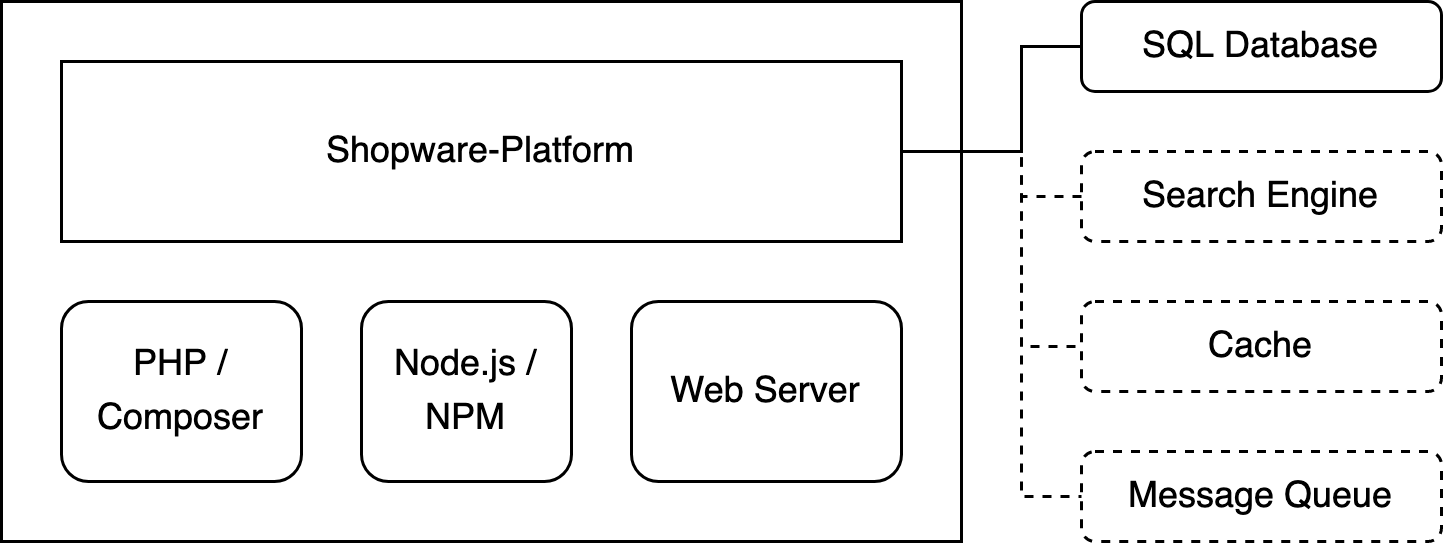
\includegraphics[width=0.6\textwidth]{images/content/shopware-requirements}
    \captioncite[Eigene Darstellung nach]{shopware-requirements}{Umgebung und Abhängigkeiten der Shopware-Platform}
    \label{fig:shopware-requirements}
\end{figure}
Shopware besteht aus einer Vielzahl von Verzeichnissen und Dateien, jede Version der Software und jedes
Shopware-basierte Projekt unterscheiden sich voneinander.
Ungeachtet von Projekt und Version gibt es jedoch einige Grundvoraussetzungen für das Ausführen von Shopware.
Die Programmiersprache PHP mit einigen Extensions und der Paketmanager Composer müssen in der ausführenden Umgebung
installiert sein.
Zusätzlich wird die Javascript-Runtime \glqq Node\grqq\ mit Paketmanager \acrshort{npm} benötigt, um das Frontend zu
bauen.
Die Software setzt außerdem eine Datenbank für den Betrieb des Shops und das Durchführen von End-to-End-Tests voraus,
und benötigt einen Webserver um aufgerufen werden zu können.
Im Live-Betrieb unterstützt die Plattform das optionale Anbinden einer Message-Queue und einer Search Engine, um viele
gleichzeitige Zugriffe von Usern verwalten zu können und das Suchen von Produkten und Herstellern für Shop-Kunden zu
ermöglichen.
Zur weiteren Optimierung der Produktions-Umgebung kann zudem ein Cache für Warenkorb-Inhalte und Nutzer-Sessions
eingeführt werden.
\footpartcite{shopware-requirements}
In Abbildung\ \ref{fig:shopware-requirements} werden die Abhängigkeiten der Shopware-Platform und die verschiedenen
Services für den Betrieb der Software aufgezeigt.
Um ein Projekt installieren und ausführen zu können, oder um Tests auf der Code-Base durchzuführen, wird also eine
Umgebung vorausgesetzt, in der die benötigten Services und Tools installiert sind.

\subsection{Auswertung von CI/CD-Tools} \label{subsec:03-concept-2}

Um die Konzeption einer \acrshort{ci}-Pipeline durchführen zu können, müssen zunächst die zur Umsetzung verfügbaren
Tools erfasst und für den Einsatz in Kundenprojekten bewertet werden.
Dabei spielen verschiedene Aspekte eine Rolle, wie die Kompatibilität mit dem bestehenden Technologie-Stack, die
Skalierbarkeit und die Benutzerfreundlichkeit.
Nachfolgend werden verschiedene Kategorien von Tools und Services die für eine \acrshort{ci}-Pipeline genutzt werden
können, vorgestellt.

\subsubsection{Version Control Systems}

Die Integration von Software wird durch \acrshort{vcs} ermöglicht.
Änderungen im Code werden hier hinzugefügt und verschiedene Versionsstände zusammengeführt.
\acrshort{vcs} somit ein integraler Bestandteil von Continuous Integration, Fowler setzt das Führen eines einzelnen
Source-Repositories voraus, welches die Software, inklusive aller Build- und Testing-Dateien, verwaltet.
\footpartcite{fowler}
Um eine vollumfängliche \acrshort{ci}-Strategie erstellen zu können, muss also die Versionskontroll-Software
inklusive dazugehöriger Services berücksichtigt werden.
Für die Konzeption wurden einige Bekannte und erprobte Anbieter von Enterprise-\acrshort{vcs} untersucht:

\begin{itemize}
    \item{
        \textbf{GitHub}:\par
        GitHub ist ein webbasierter Hosting-Service für Versionierung mit Git.
        Es bietet alle verteilten Versionskontroll- und Quellcodeverwaltungsfunktionen von Git sowie einige
        eigene Funktionen.
        Es bietet Zugriffskontrolle und mehrere Kollaborationsfunktionen wie Aufgabenverwaltung, Fehlerverfolgung und
        Feature-Requests für Projekte.
        GitHub bietet sowohl Pläne für private Repositorys als auch kostenlose Konten, die normalerweise verwendet
        werden, um Open-Source-Softwareprojekte zu hosten.
        Der Service bietet außerdem \acrshort{ci}-Tools und Pipeline-Verwaltung an.
        Als Managed Service kümmert sich GitHub um die Wartung der Infrastruktur.\footpartcite{github}
    }

    \item{
        \textbf{GitLab}:\par
        GitLab ist ein webbasiertes \acrshort{vcs}-Tool, welches einen Git-Repository-Manager bereitstellt.
        Der Service ist vergleichbar mit GitHub und bietet viele ähnliche Funktionen, wie Issue-Tracking,
        kontinuierliche Integration und Deployment-Pipelines, sowie eine integrierte Wiki-Funktion für die
        Dokumentation.
        Es wird unter einer Open-Source-Lizenz vertrieben und eine Self-Managed-Version ermöglicht es,
        GitLab auf eigenen Servern zu installieren und zu verwalten.
        Dies bietet mehr Kontrolle über die Daten und die Möglichkeit, die Plattform an spezifische Bedürfnisse
        anzupassen.\footpartcite{gitlab}
    }

    \item{
        \textbf{Bitbucket}:\par
        Bitbucket ist ein weiteres webbasiertes Tool zur Verwaltung von \acrshort{vcs}, welches sowohl von
        kommerziellen als auch von kostenlosen Konten genutzt wird.
        Es wird von der Firma Atlassian betrieben und ermöglicht das Hosting von Git- und Mercurial-Repositorys.
        Bitbucket integriert auch mit anderen Atlassian-Produkten wie Jira und Confluence.
        Es bietet Funktionen wie Pull-Requests für Code-Reviews und Inline-Kommentare.
        Bitbucket bietet sowohl Managed als auch Self-Hosted-Optionen.\footpartcite{bitbucket}
    }

    \item{
        \textbf{SourceForge}:\par
        SourceForge ist eine Open-Source \acrshort{vcs}-Lösung, welche sowohl Git als auch Mercurial unterstützt.
        Die Plattform kann sowohl zur Versionskontrolle als auch für das Ausliefern von Software verwendet werden,
        wobei diese oft für Open-Source-Projekte genutzt wird.
        SourceForge ist webbasiert und bietet den direkten Download von einer Vielzahl von Software-Projekten an.
        \footpartcite{sourceforge}
    }
\end{itemize}

\subsubsection{Pipeline- und Test-Runners}

Um die in einer Versionskontroll-Software eingeführten Code-Änderungen automatisiert bauen, testen und ausliefern zu
können, wird eine ausführende Umgebung für diese Prozesse benötigt.
Für diese Problemstellung gibt es Pipelines, welche zum Ausführen von Befehlen und Prozessen zur
automatischen Integration und dem Testen von Code genutzt werden.\footpartcite[2]{benefits-challenges}
Viele \acrshort{vcs}-Anbieter haben bereits eine Pipeline-Lösung in ihrem System integriert und bieten die
Hardware-Ressourcen zum Ausführen der Pipelines an.
Neben den eingebauten Pipeline-Services der Enterprise-Anbieter gibt es einige eigenständige Tools, manche davon
Open-Source-Projekte, welche Teils selbst gehostet werden müssen.
Nachfolgend werden einige dieser Build-automations-Tools im Hinblick auf den Einsatz in der zu entwickelnden Strategie
untersucht:

\begin{itemize}
    \item{
        \textbf{GitHub Actions}:\par
        ...
    }

    \item{
        \textbf{GitLab CI/CD}:\par
        ...
    }

    \item{
        \textbf{Bitbucket Pipelines}:\par
        ...
    }

    \item{
        \textbf{Jenkins}:\par
        ...
    }

    \item{
        \textbf{Travis CI}:\par
        ...
    }

    \item{
        \textbf{Circle CI}:\par
        ...
    }
\end{itemize}

\subsubsection{Testing-Tools}

\subsubsection{Static-Code-Analysis-Tools}

\subsubsection{Dependency Trackers}

\subsubsection{Weitere Tools und Services}

\subsection{Konzeption der CI-Strategie} \label{subsec:03-concept-3}

\clearpage
